\section{Implementation \& Training}
\label{sec-implementation-and-training}




In our experiment, we are forced to collect the training dataset on our own instead of using public datasets, as there is no publicly available image dataset built for shoulder-surfing to the best of our knowledge, and because of the uniqueness of our application, i.e. blurriness, targeting characters, working with burst mode snapshots, etc., we cannot find any publicly avaliable substitudes.
%Modern network architectures work with naturally obtained images, e.g. ordinary photos, satellite images, scanned documents, YouTube videos, etc. where the images are well focused and captured within the imaging ability of the camera, with the objects of interest, e.g. the face or the printed word, at least visible to the naked eye. and we apply the SR algorithms to reduce noise and refine details, like repainting texture and refining edges. However, as emphasized above, in our application we face images that is extremely blurred and distorted, due to the extreme circumstances when the photos are taken, and it is impossible to tell from each single picture whether a stroke of a character really belongs here, as it's equally possible that this line is a distorted mixture of multiple lines or is a mutilated part of a longer stroke. These are the reasons why our work does not choose datasets that are publicly available, and collect data by ourselves--as it will completely defeat the purpose if we turn to these datasets. And this also explains why we failed in trying to get comparable results with other SR architectures we use as baselines, as these networks are designed for another purpose and they hardly ever faced such distorted and blurred images.

%Note that different lenses have different photographing abilities and blurring patterns, so the model has to be trained for each phone model.
 %To reduce calculation and better align the images with the ground truth, in the training data collection phase we drew a box around the text on the victim's screen, replacing the edges of the phone for alignment and cropping in the alignment step (as shown in Figure~\ref{fig-training}), but our system works perfectly without it.

\subsection{Experiment Setting}
\label{sec-experiment-setting}
Our experiment consists of 2 smartphones, one for the attacker and one the victim. Their distance is between 1 and 2 meters for traditional lens and 5 to 7.5 meters for optical lens. Both phones are fixed to stands to keep them completely still, but the lenses with optical zoom will shift slightly time to time, which can simulate a handheld situation. An app runs inside the attacker's phone, taking photos in burst mode repeatedly (no more than 20 photos per burst), and another app runs inside the victim's phone, displaying random characters with random fonts and colors. The characters are selected from commonly used Chinese characters with 5 to 10 strokes and the English alphabet, and we divide this character assemble into training and testing subsets. As the English characters are apparently easier to classify and reconstruct for the networks, the experiments testing the performance of the network will be performed only on Chinese characters, but it is our observation that our system works on English characters as well as Chinese characters. Screenshots were taken in the victim's phone as ground truth for training and evaluation. An illustration of our experimental setting is displayed in Fig.~\ref{illustration_of_system}.
\begin{figure}
	\centering
	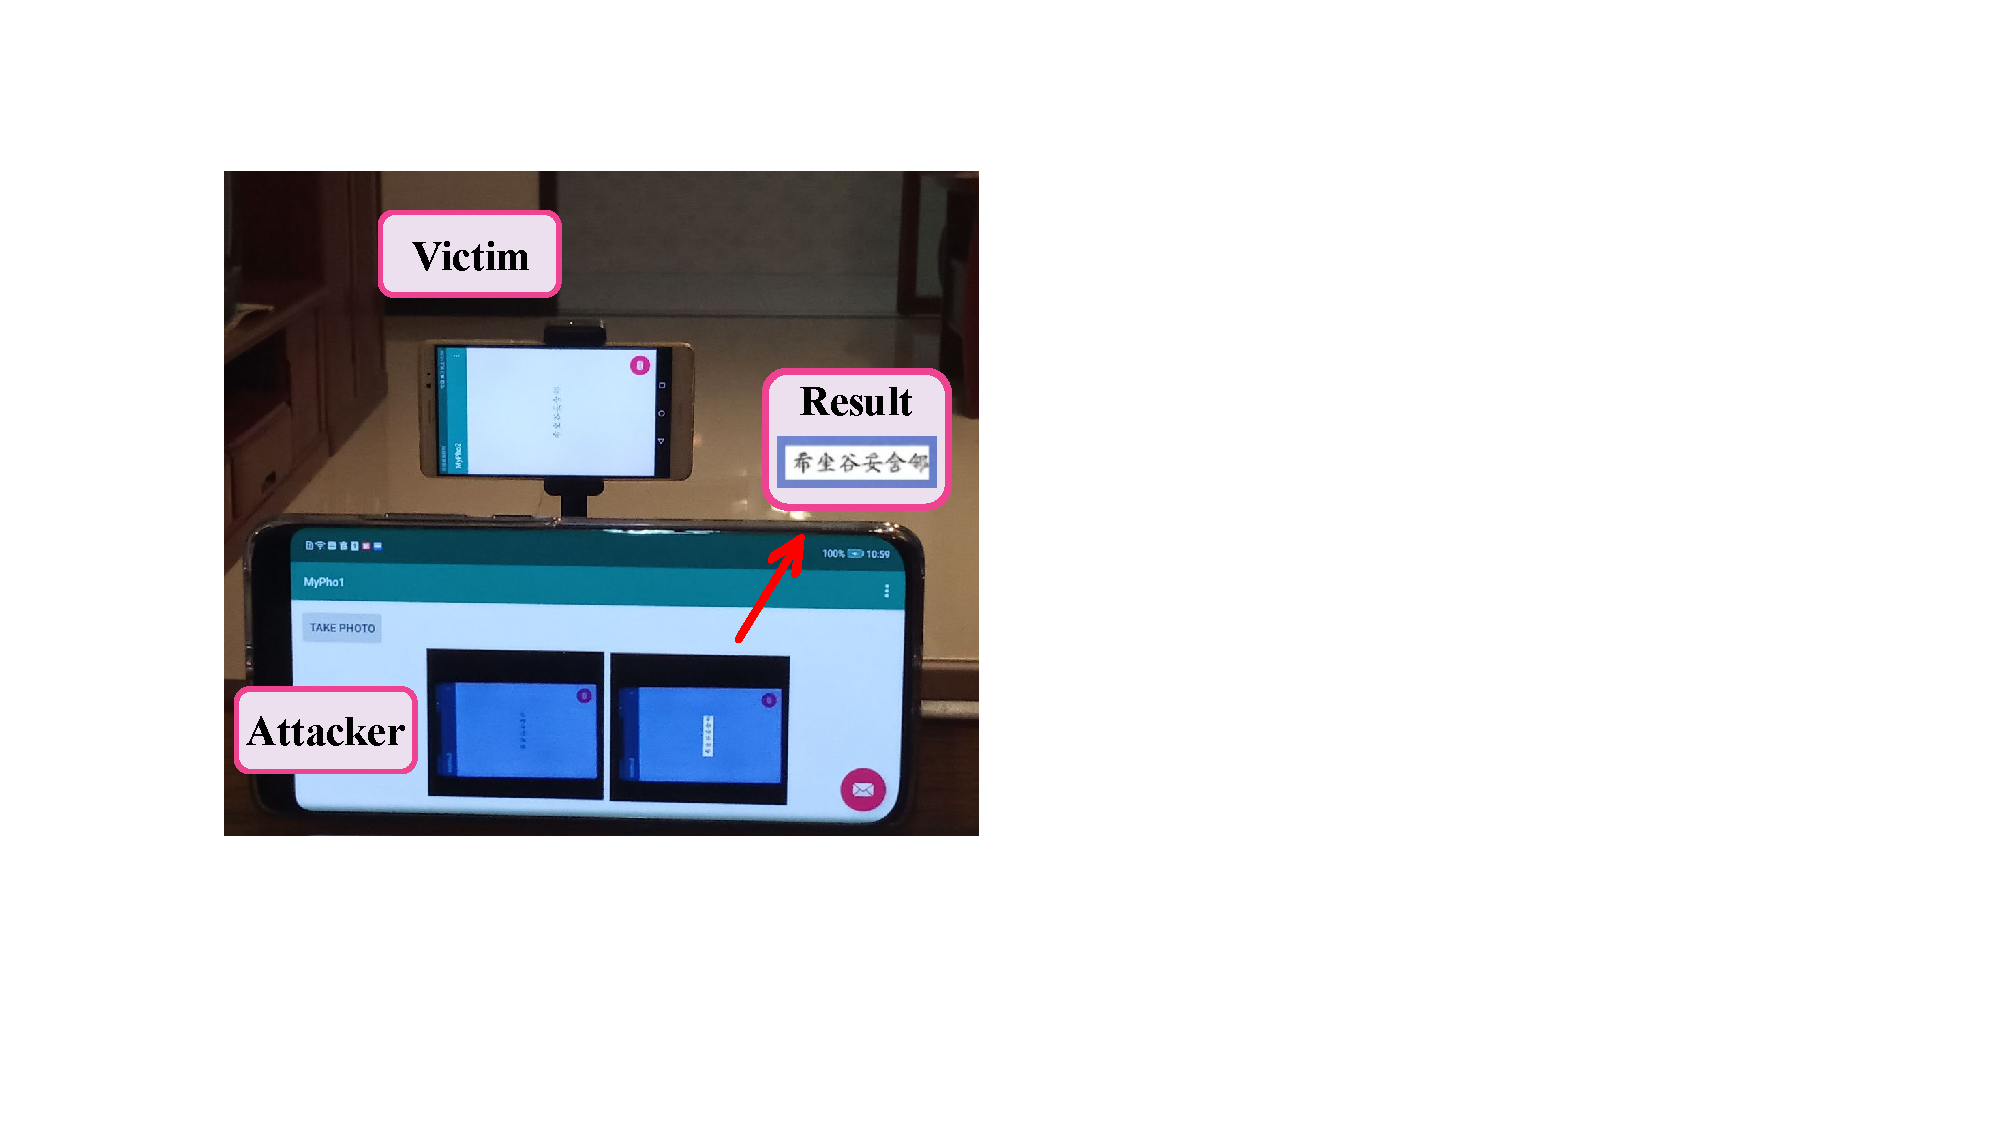
\includegraphics[width=0.80\linewidth]{pic/setup.pdf}
    \caption{Illustration of our experimental setting (distance between phones is shortened for demonstration).}
	\label{illustration_of_system}
\end{figure}
% \begin{figure}
%   \centering
%      \centering
%      \subfigure[Experiment setting. Distance between phones are shortened for demonstration.]{
%          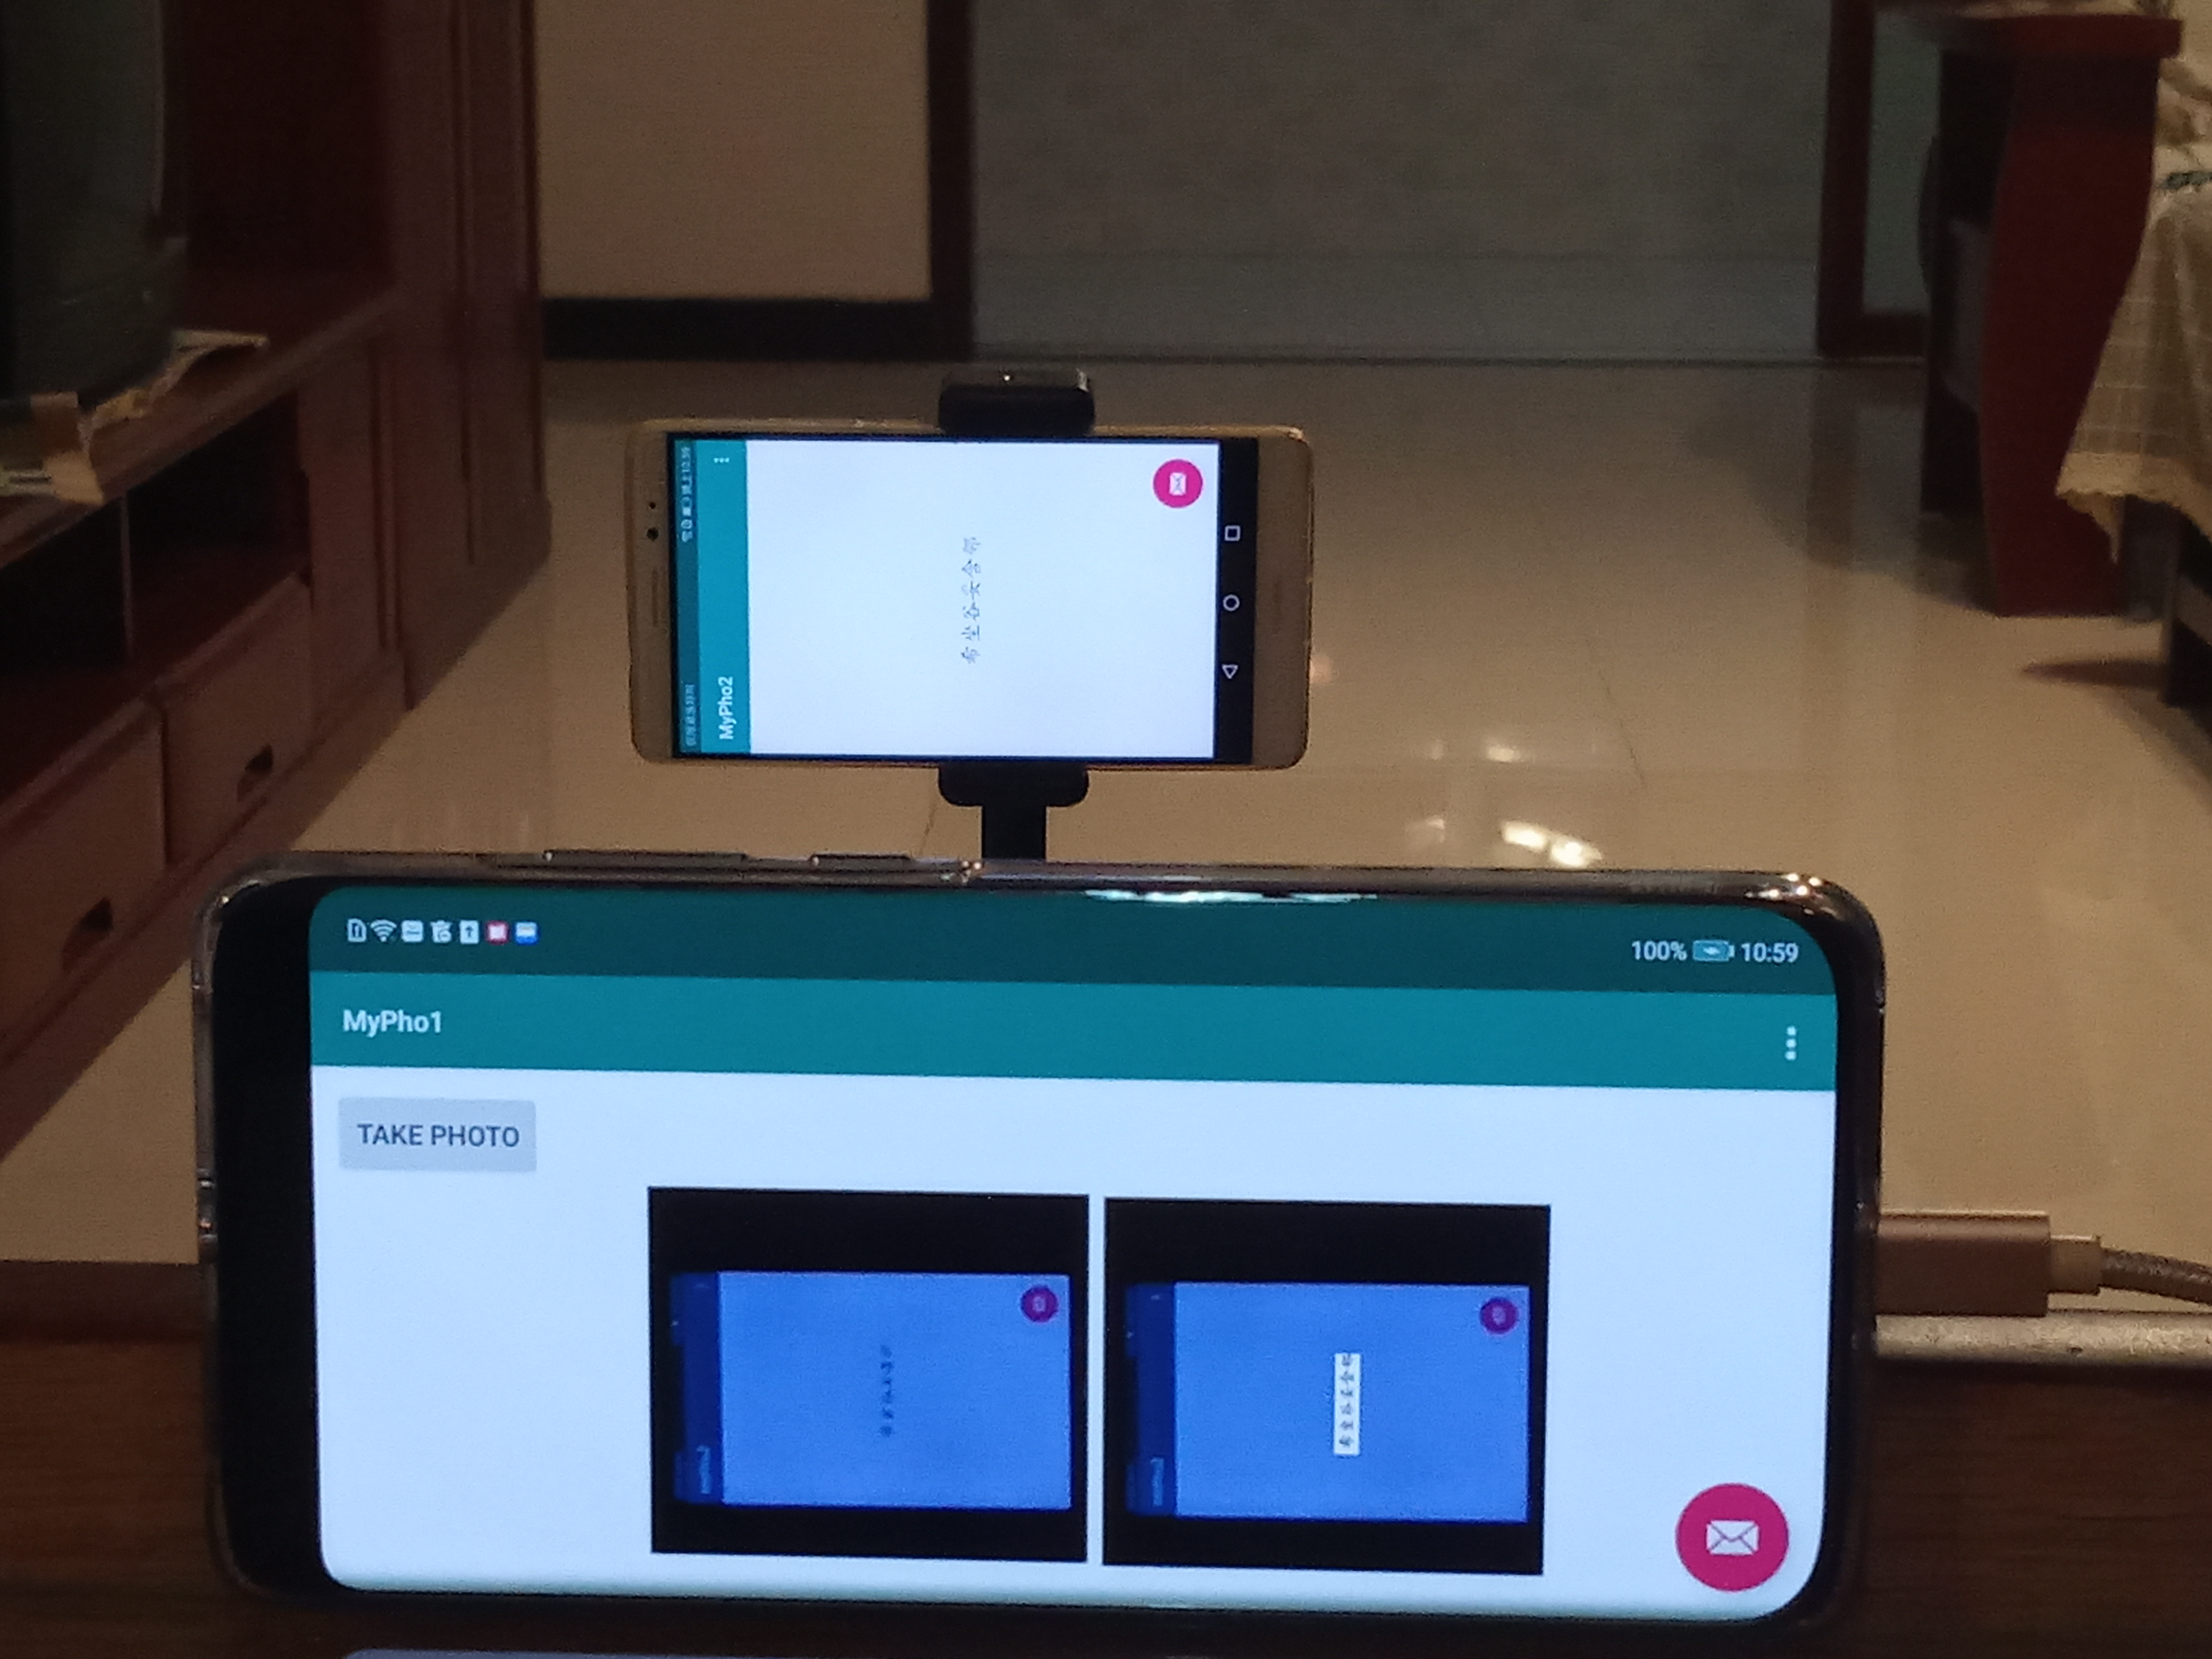
\includegraphics[width=0.5\textwidth]{pic/exp1.jpg}
%          \label{fig-exp1}
%          }
%    \subfigure[screenshot from attacker's phone(SRPeek system).]{
%          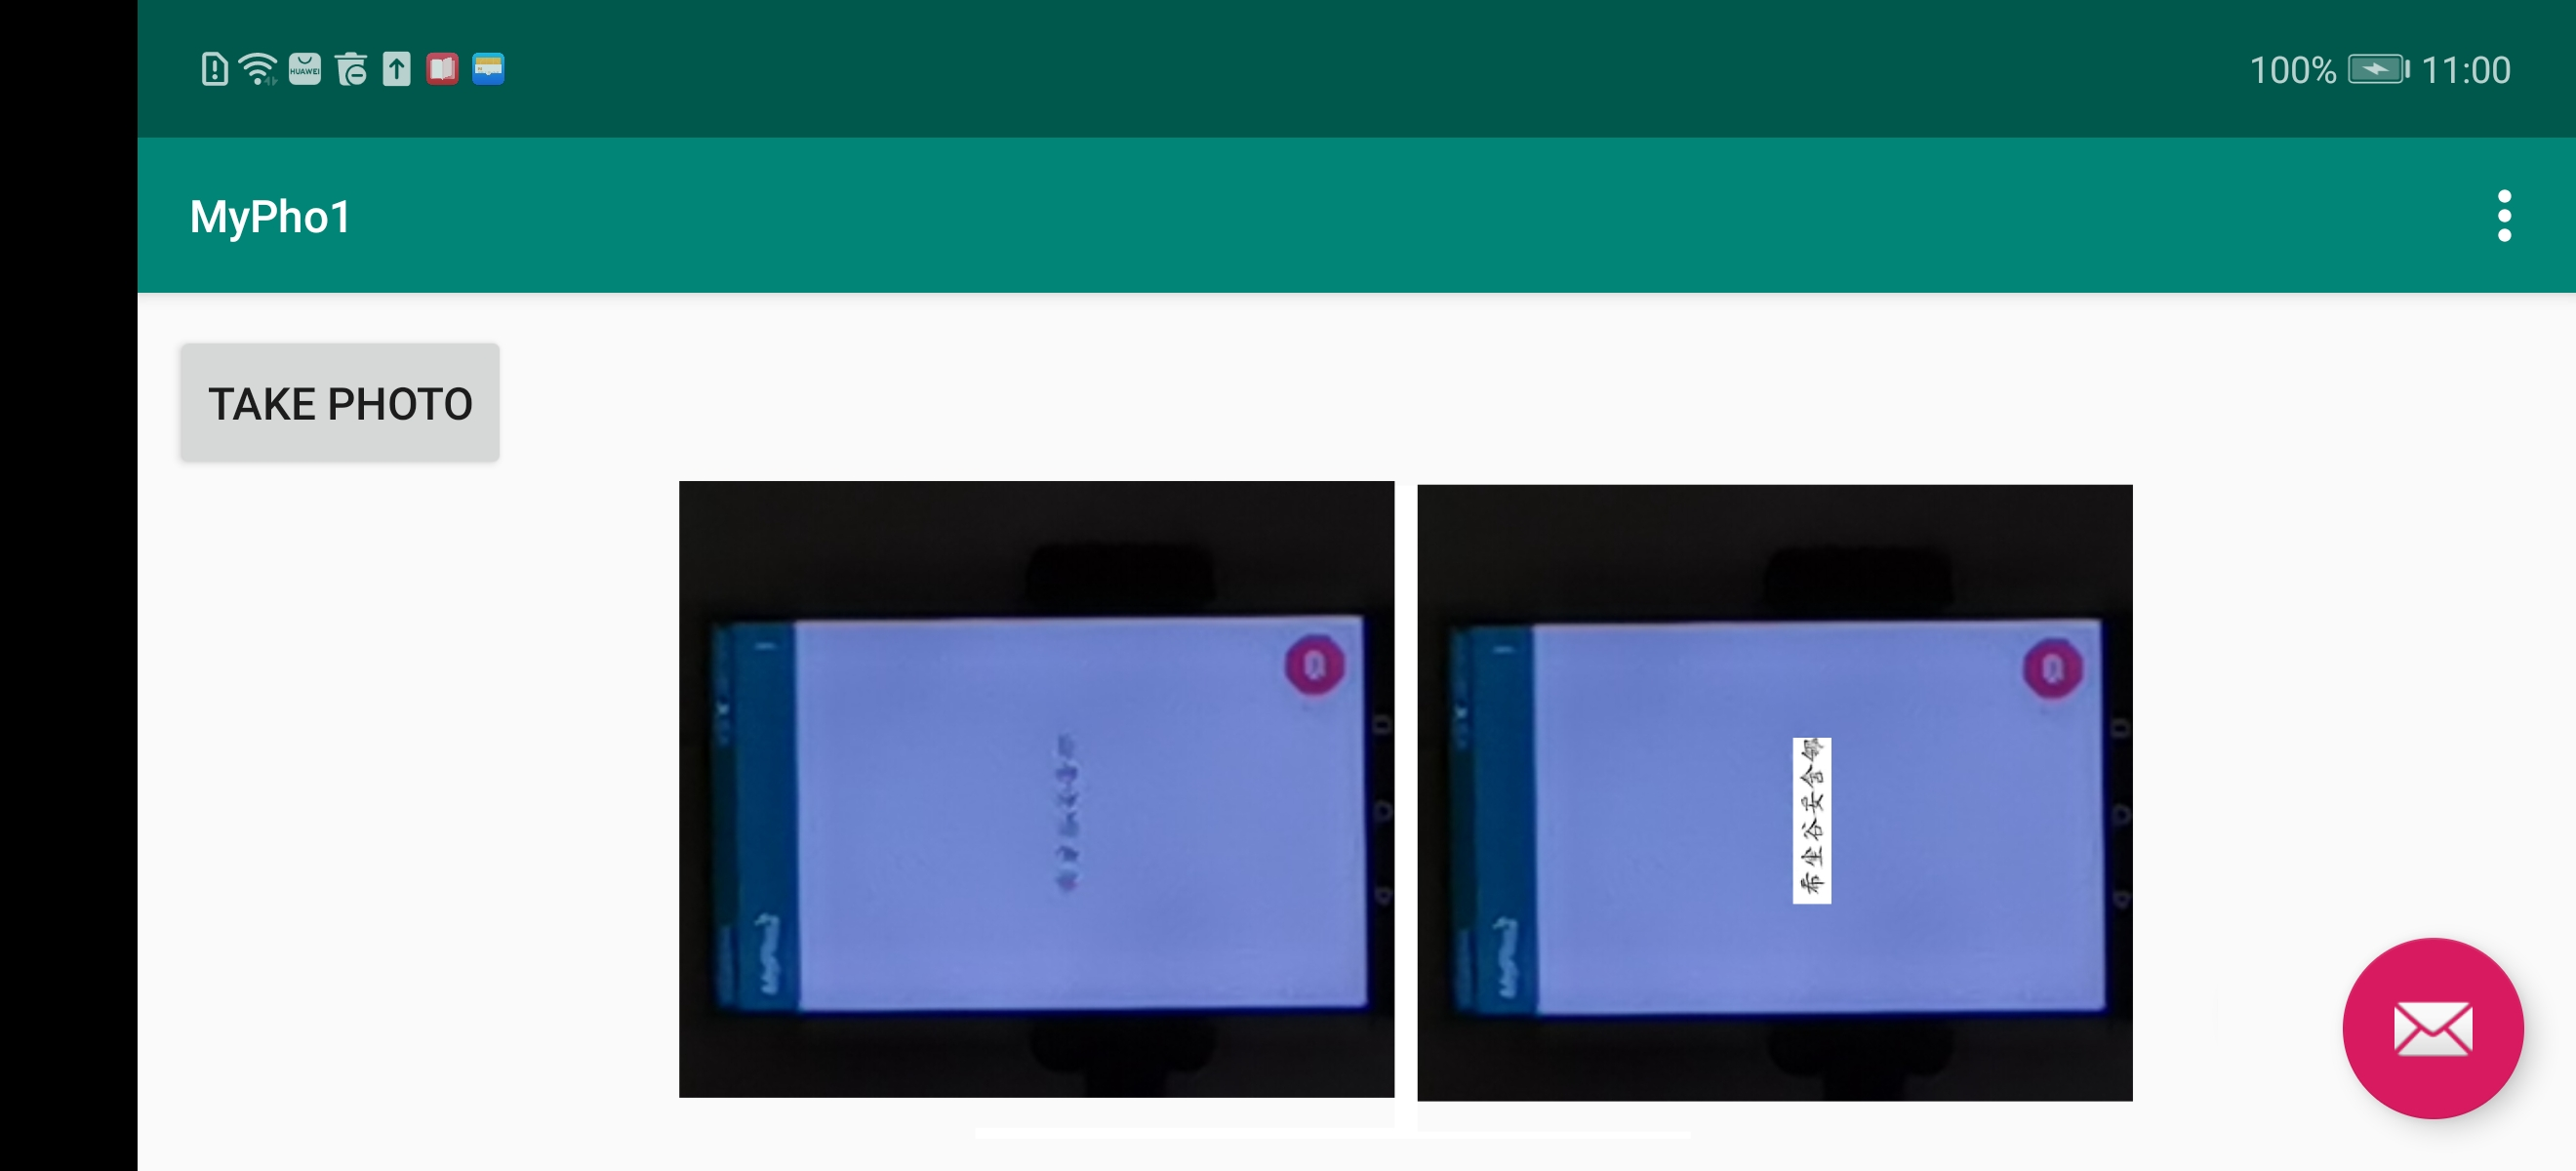
\includegraphics[width=0.5\textwidth]{pic/exp2.jpg}
%          \label{fig-exp2}
%          }
%    \subfigure[screenshot from victim's phone.]{
%          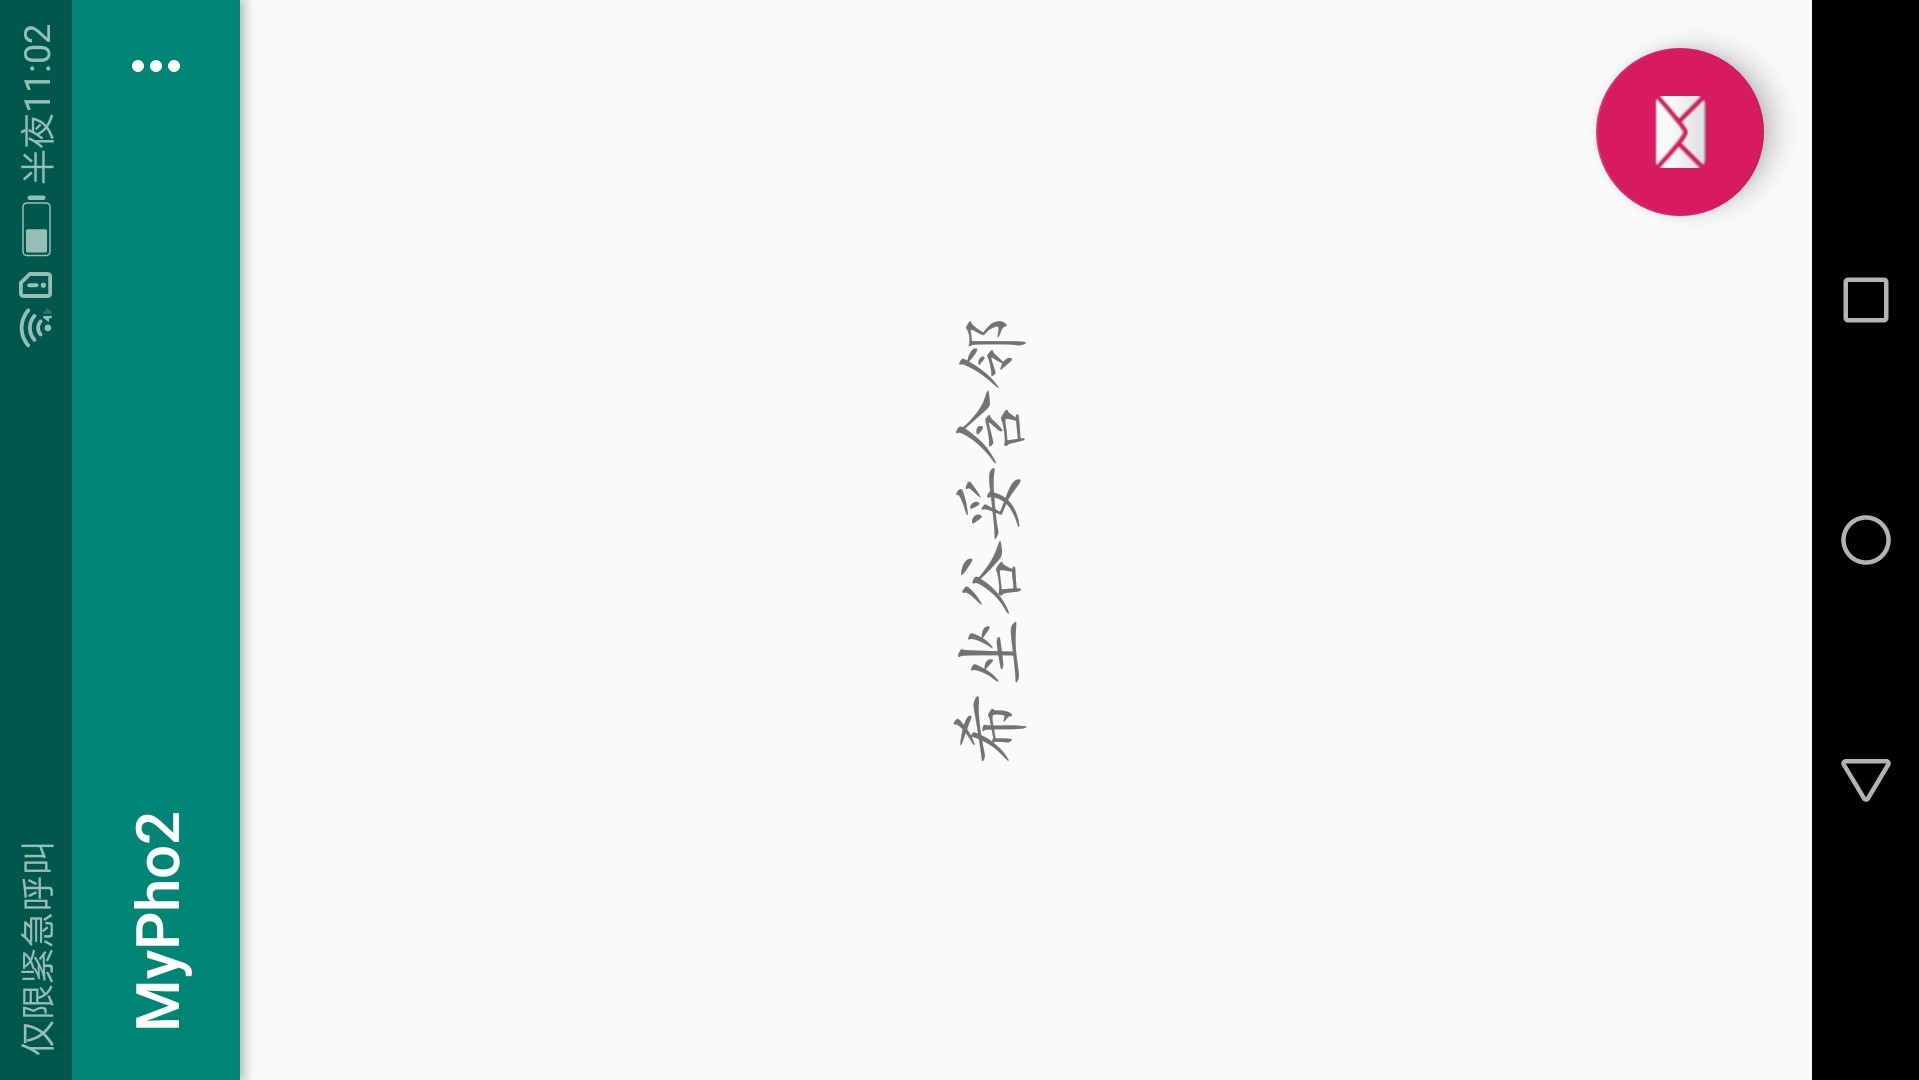
\includegraphics[width=0.5\textwidth]{pic/exp3.jpg}
%          \label{fig-exp3}
%          }
%      \caption{Illustration of our experimental setting.}
%      \label{fig-experiment}
% \end{figure}

The data was collected at different times of the day and night, with different illumination and at different positions and angles(tilting no more than 30 degrees). We collected 800,000 images in this way with a Redmi6A phone (which possess a camera with 130 million pixels), modifying these environmental parameters every 2,000 images. This process is extremely time-consuming, but the data amount is crucial in our experiment, as slight variations of the environment will cause drastic changes in the features extracted from the characters, and only by covering the variations in each of the environmental parameters in the training data can the system successfully function in different scenarios.

\subsection{Model Specifications}
It is our observation that cameras in different phones display different patterns of distortion when performing the shoulder-surfing experiment, and apparently, images captured from a phone with weaker abilities (less pixels, less range of focus, worn lenses, etc.) will need a stronger, more complex model to extract the features. Thus, the specifications of our model are only for reference and may not work when reproduced on another phone. Also, we may need to repeat the data collection and training phases when switching to another phone model.

Our model accepts any number of images per burst, but it can only process a patch of 9$\times$9 pixels(not necessarily containing whole characters, as it functions at the strokes level) at a time. We expect that characters should be upright(the attacker can simply spin his phone). The model consists of 5 blocks described in the previous section. In each block, feature maps from the previous layer are passed through a single convolutional layer with 32 channels of feature maps as output. the 20$\times$32 feature maps are then merged horizontally with the max-min-average process, and the output is 5$\times$32 channels. Simultaneously, the original input images are processed again with a single convolutional layer with 32 channels output, and stacked with the former 5$\times$32 channels to form a dataflow of 6$\times$32 channels for each one of the images. These channels are finally passed through a single convolutional layer, outputting 32 channels per image for the next block. The kernels in each convolutional layer is 3$\times$3. We also insert LeakyReLU and Batch Normalization processes after each convolutional layer, and 2 upsampling layers between the 5 blocks. A single 1$\times$1 convolutional layer is placed after the 5 blocks with a single channel as output to form the final output layer. This model consists of approximately 200,000 parameters and a complexity of about 400,000 FLOPs. As a light-weighted model, it makes a prediction within 0.1 seconds on a Tesla K80 GPU over a 9$\times$9 patch, and when implemented on a smartphone, the human user can recognize a character within 2 seconds of processing time.